\chapter{Ons voedsel produceren}\label{ch:g6:producing-our-food}

Niets op je ontbijttafel is in het wild gevonden. De tarwe van het brood
is veredeld en verbouwd; de \omterm{def:g2:animals-grow-up:born}{melk} kwam van kuddes die daarvoor gehouden
worden; de yoghurt is uit die \omterm{def:g2:animals-grow-up:born}{melk} \emph{gemaakt} door miljarden levende
werkers die te klein zijn om te zien. Mensen voeden zichzelf door \omterm{def:g6:exploring-our-environment:components}{levende
wezens} te beheren --- ze te telen, ze te houden, en sommige van de
allerkleinste aan het werk te zetten. Dit hoofdstuk maakt een rondgang
door de voedselwerkplaats.

\section{Telen en houden}

\begin{definition}[Gewassen en vee]\label{def:g6:producing-our-food:farming}
De menselijke voedselproductie beheert \omterm{def:g6:exploring-our-environment:components}{levende wezens} op twee
verdiepingen van de materiekringloop:
\begin{itemize}
  \item de \emph{akkerbouw}\index{gewas}: \omterm{def:g5:food-webs:roles}{producenten} beheren --- tarwe,
        aardappelen, groente, fruit --- om hun \omterm{def:g6:plants-are-producers:matter}{organische materie}
        (\cref{prop:g6:plants-are-producers:produce});
  \item de \emph{veehouderij}\index{vee}: \omterm{def:g5:food-webs:roles}{consumenten} beheren ---
        runderen, schapen, varkens, kippen --- om hun \omterm{def:g6:matter-from-food:production}{materieproductie}
        (\cref{def:g6:matter-from-food:production}): \omterm{def:g2:animals-grow-up:born}{melk}, vlees,
        eieren, wol.
\end{itemize}
Boeren beheren de \omterm{def:g6:exploring-our-environment:conditions}{omstandigheden} die dit boek steeds tegenkomt:
bodemmineralen voor de gewassen (\cref{rem:g4:what-plants-need:soil}),
voer voor de \omterm{def:g1:animals-around-us:animal}{dieren} --- de hele boekhouding van
\cref{pb:g6:matter-from-food:1}, met opzet gevoerd.
\end{definition}

\begin{example}[Wat een tarweakker is]\label{ex:g6:producing-our-food:wheat}
Een tarweakker is een beheerde \omterm{def:g6:exploring-our-environment:components}{omgeving}
(\cref{prop:g5:people-and-nature:managed}) die op één \omterm{def:g5:food-webs:roles}{producent} is
afgestemd: de bodem aangevuld en losgemaakt voor haar \omterm{def:g1:plants-around-us:parts}{wortels}, het zaaien
afgestemd op de warmte uit \cref{prop:g2:from-seed-to-plant:needs},
onkruid --- rivaliserende kolonisten uit
\cref{ch:g6:how-plants-spread} --- buiten gehouden. De oogst is de
zaadvoorraad van de \omterm{def:g1:plants-around-us:plant}{plant}: graan, de lunchpakketten van een miljoen
tarweplanten die nooit gezaaid zullen worden, omgeleid naar bakkerijen.
\end{example}

\begin{remark}[Elk voedsel is een stadium van een levenscyclus]\label{rem:g6:producing-our-food:stage}
Lees elk voedsel biologisch en het is een orgaan of stadium van een of
ander organisme: graan en bonen zijn zaadvoorraden; aardappelen knollen;
appels \omterm{prop:g3:flowers-fruits-seeds:transform}{vruchten} die gebouwd zijn om opgegeten te worden
(\cref{exo:g6:how-plants-spread:12}); \omterm{def:g2:animals-grow-up:born}{melk} is moederzorg van een zoogdier
(\cref{def:g2:animals-grow-up:born}); een \omterm{def:g2:animals-grow-up:born}{ei} is een ingepakte
kraamkamer. Voedselproductie is de kunst om levenscycli zo te beheren dat
hun proviand op onze tafel belandt.
\end{remark}

\section{De onzichtbare beroepsbevolking: voedsel gemaakt door microben}

\begin{definition}[Gisting]\label{def:g6:producing-our-food:fermentation}
Sommige voedingsmiddelen worden gemaakt door \omterm{def:g6:exploring-our-environment:components}{levende wezens} die te klein
zijn om te zien --- \emph{microben}\index{microbe (voedsel)} --- op een
grondstof te zetten. Hun eten zet die om: die omzetting heet
\emph{gisting}\index{gisting}, en mensen laten haar al duizenden jaren
draaien, lang voordat iemand wist dat de werkers bestonden.
\end{definition}

\begin{example}[Brood rijst]\label{ex:g6:producing-our-food:bread}
Rauw brooddeeg is \omterm{def:g3:flowers-fruits-seeds:parts}{bloem} en water --- plus \emph{gist}\index{gist}, een
eencellige \omterm{def:g6:decomposers-and-soil:decomposers}{schimmel} (\cref{rem:g5:first-look-at-cells:onecelled} kwam
zulke levens al tegen). De \omterm{ex:g6:producing-our-food:bread}{gist} voedt zich met de suikers van de \omterm{def:g3:flowers-fruits-seeds:parts}{bloem} en
geeft een gas af; de bellen van dat gas, gevangen in het rekbare deeg,
blazen het op --- de bakker noemt dat rijzen. De hitte van de oven maakt
daarna een eind aan de dienst van de werkers en zet hun werk vast: de
gaten in het kruim zijn de handtekening van de \omterm{ex:g6:producing-our-food:bread}{gist}.
\end{example}

\begin{omfigure}
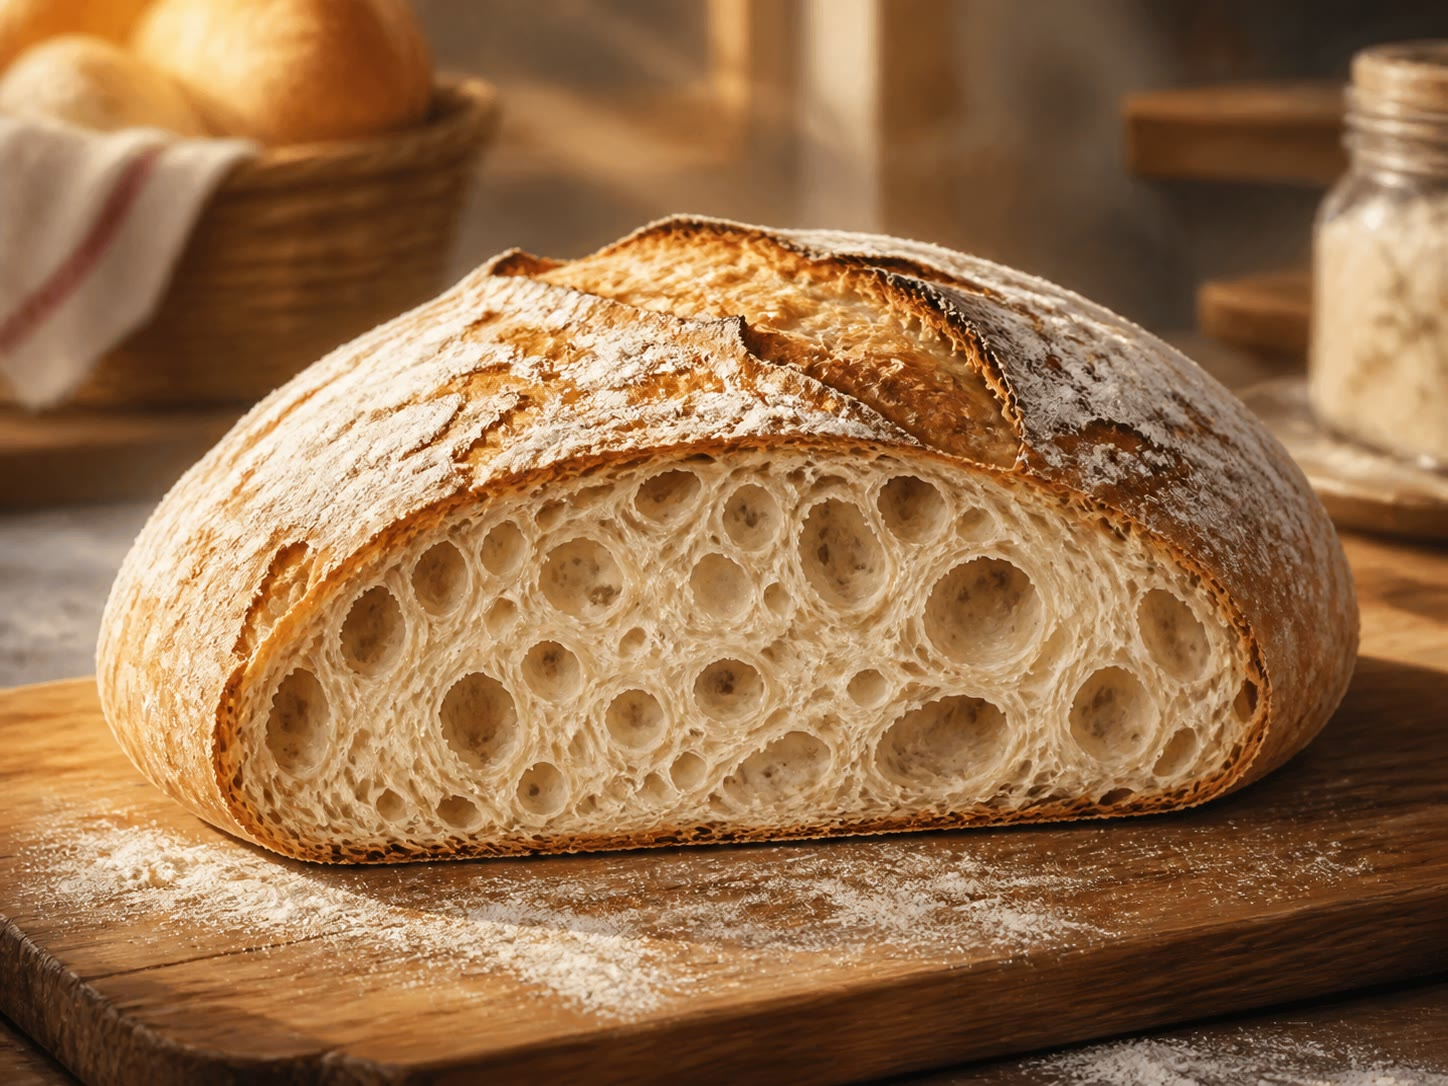
\includegraphics[width=0.58\linewidth]{images/book1/ai/g6-food-bread.jpg}

{\small De handtekening van de beroepsbevolking, ter plekke gebakken:
elk gat in het kruim is een bel die de \omterm{ex:g6:producing-our-food:bread}{gist} geblazen heeft.}
\end{omfigure}

\begin{example}[Melk wordt yoghurt en kaas]\label{ex:g6:producing-our-food:yogurt}
Warme \omterm{def:g2:animals-grow-up:born}{melk} waarin de juiste \omterm{def:g6:producing-our-food:fermentation}{microben} gezet zijn, dikt 's nachts in tot
yoghurt: de werkers voeden zich met de suiker van de \omterm{def:g2:animals-grow-up:born}{melk} en geven een
zuur af, en dat zuur laat de \omterm{def:g2:animals-grow-up:born}{melk} stollen --- de frisse zure smaak
\emph{is} het zuur. Kaas begint net zo en gaat dan verder: de wrongel
wordt geperst, gezouten en maandenlang gerijpt, terwijl de \omterm{def:g6:producing-our-food:fermentation}{microben}
tijdens dat rijpen doorwerken --- de gaten, de korst en de kracht van de
geur van een kaas zijn het logboek van hun lange dienst.
\end{example}

\begin{remark}[Nuttige en schadelijke microben]\label{rem:g6:producing-our-food:goodbad}
De \omterm{def:g1:healthy-habits:germs}{ziektekiemen} uit \cref{def:g1:healthy-habits:germs} leerden ons
voorzichtig te zijn met \omterm{def:g6:producing-our-food:fermentation}{microben}; dit hoofdstuk voegt de andere helft
toe: \emph{gekozen} \omterm{def:g6:producing-our-food:fermentation}{microben}, die in \emph{beheerste} \omterm{def:g6:exploring-our-environment:conditions}{omstandigheden}
werken, horen bij onze oudste werknemers --- in brood, yoghurt, kaas en
het azijnvat. Het vak is altijd hetzelfde: verwelkom de gekozen werkers,
en houd de \omterm{def:g6:exploring-our-environment:conditions}{omstandigheden} zo dat ze hun passen en de bedervers niet.
Zouten, koelen, drogen en koken zijn allemaal manieren om ongewenste
\omterm{def:g6:producing-our-food:fermentation}{microben} hun \omterm{def:g6:exploring-our-environment:conditions}{omstandigheden} te weigeren
(\cref{prop:g6:decomposers-and-soil:speed} werkt op een ham precies zoals
op een bladerhoop).
\end{remark}

\section{Van akker tot tafel, eerlijk gezegd}

\begin{proposition}[De kosten op tafel]\label{prop:g6:producing-our-food:costs}
Elk bord is een opbrengst van beheerd land en beheerde \omterm{def:g6:exploring-our-environment:components}{levende wezens}, en
draagt hun rekenkunde met zich mee:
\begin{itemize}
  \item plantaardig voedsel komt één verdieping vanaf het licht;
        dierlijk voedsel gaat eerst via een \omterm{def:g5:food-webs:roles}{consument} en betaalt de tol
        van \cref{prop:g6:matter-from-food:losses}
        (\cref{exo:g6:matter-from-food:12});
  \item duurzame productie moet de drie regels van
        \cref{prop:g5:people-and-nature:lasting} aanhouden --- voed de
        bodem, houd de helpers, neem niet sneller dan de vernieuwing;
  \item en verspilling maakt alles ongedaan: weggegooid voedsel heeft
        zijn land, water en werk voor niemand uitgegeven.
\end{itemize}
\end{proposition}
\admitted

\begin{method}[Het verhaal van een voedingsmiddel lezen]\label{met:g6:producing-our-food:read}
Voor elk voedingsmiddel in de keuken:
\begin{enumerate}
  \item noem het organisme en het orgaan of stadium dat het is
        (\cref{rem:g6:producing-our-food:stage});
  \item plaats het in de kringloop: materie van een \omterm{def:g5:food-webs:roles}{producent}, product
        van een \omterm{def:g5:food-webs:roles}{consument}, of door \omterm{def:g6:producing-our-food:fermentation}{microben} gemaakt?
  \item is het door \omterm{def:g6:producing-our-food:fermentation}{microben} gemaakt, noem dan de grondstof en wat de
        werkers veranderd hebben;
  \item volg het terug naar zijn \omterm{def:g1:plants-around-us:parts}{blad}
        (\cref{met:g6:plants-are-producers:trace}) --- het spoor eindigt
        nog steeds altijd in het licht.
\end{enumerate}
\end{method}

\begin{example}[De methode bij het ontbijt]\label{ex:g6:producing-our-food:breakfast}
Yoghurt, volgens de methode: (1) \omterm{def:g2:animals-grow-up:born}{melk} --- een product van de moederzorg
van een koe --- omgezet; (2) product van een \omterm{def:g5:food-webs:roles}{consument}, door \omterm{def:g6:producing-our-food:fermentation}{microben}
afgemaakt; (3) grondstof \omterm{def:g2:animals-grow-up:born}{melk}, de werkers hebben haar zuur gemaakt en
laten stollen; (4) \omterm{def:g2:animals-grow-up:born}{melk} van de koe, koe van gras, gras van licht. Drie
organismen en een beroepsbevolking van miljarden, in één klein bakje.
\end{example}

\section{Oefeningen}

\begin{exercise}[$\star$]\label{exo:g6:producing-our-food:1}
Omschrijf \omterm{def:g6:producing-our-food:farming}{akkerbouw} en \omterm{def:g6:producing-our-food:farming}{veehouderij}, en noem bij elk de verdieping van de
materiekringloop die ze beheert.
\end{exercise}

\begin{exercise}[$\star$]\label{exo:g6:producing-our-food:2}
Noem bij elk voedingsmiddel het organisme en het orgaan of stadium:
graan, aardappel, appel, \omterm{def:g2:animals-grow-up:born}{melk}, \omterm{def:g2:animals-grow-up:born}{ei}.
\end{exercise}

\begin{exercise}[$\star$]\label{exo:g6:producing-our-food:3}
Wat is \omterm{def:g6:producing-our-food:fermentation}{gisting}? Noem twee gegiste voedingsmiddelen en hun grondstoffen.
\end{exercise}

\begin{exercise}[$\star$]\label{exo:g6:producing-our-food:4}
Vertel waarom brood rijst: de werker, zijn voedsel, wat hij afgeeft, en
wat de oven doet.
\end{exercise}

\begin{exercise}[$\star$]\label{exo:g6:producing-our-food:5}
Wat laat \omterm{def:g2:animals-grow-up:born}{melk} tot yoghurt stollen, en waar komt de zure smaak vandaan?
\end{exercise}

\begin{exercise}[$\star$]\label{exo:g6:producing-our-food:6}
Geef drie manieren om ongewenste \omterm{def:g6:producing-our-food:fermentation}{microben} hun \omterm{def:g6:exploring-our-environment:conditions}{omstandigheden} te weigeren,
uit \cref{rem:g6:producing-our-food:goodbad}.
\end{exercise}

\begin{exercise}[$\star\star$]\label{exo:g6:producing-our-food:7}
Een tarweakker beheert met opzet elke behoefte uit
\cref{prop:g4:what-plants-need:needs}. Koppel elke behoefte aan de
handeling van de boer uit \cref{ex:g6:producing-our-food:wheat}.
\end{exercise}

\begin{exercise}[$\star\star$]\label{exo:g6:producing-our-food:8}
Laat \cref{met:g6:producing-our-food:read} stap voor stap lopen over kaas.
\end{exercise}

\begin{exercise}[$\star\star$]\label{exo:g6:producing-our-food:9}
Waarom houdt koelen voedsel goed --- en waarom vertraagt diezelfde kou
een composthoop? Eén beginsel, twee keukens: noem het.
\end{exercise}

\begin{exercise}[$\star\star$]\label{exo:g6:producing-our-food:10}
Breng \cref{def:g1:healthy-habits:germs} in overeenstemming met dit
hoofdstuk: hoe kunnen \omterm{def:g6:producing-our-food:fermentation}{microben} tegelijk de vijand van het handen wassen
en de beroepsbevolking van de yoghurt zijn?
\end{exercise}

\begin{exercise}[$\star\star$]\label{exo:g6:producing-our-food:11}
Leg met \cref{prop:g6:producing-our-food:costs} uit waarom een weggegooid
broodje ham meer verspilt dan hetzelfde gewicht weggegooid brood.
\end{exercise}

\begin{exercise}[$\star\star\star$]\label{exo:g6:producing-our-food:12}
Duizenden jaren lang lieten bakkers en brouwers \omterm{def:g6:producing-our-food:fermentation}{gisting} draaien zonder te
weten dat \omterm{def:g6:producing-our-food:fermentation}{microben} bestonden. Wat beheerden zij eigenlijk, in de termen
van \cref{prop:g6:exploring-our-environment:decide} --- en waarom werkten
hun recepten toch?
\end{exercise}

\section{Probleem: De bakkerij van de klas}

\begin{problem}[{Weekendprobleem --- één baksel brood, gevolgd van zaad
tot snee}]\label{pb:g6:producing-our-food:1}
Voor de schoolmarkt bakt de klas zelf brood --- en houdt haar
biologieschrift open van het bezoek aan de tarweakker in juli tot de
broden in november.

\medskip\noindent\textbf{Deel I --- De akker (juli).}
\begin{enumerate}
  \item De boer laat de rijpe tarwe zien: ``de oogst zijn de
        lunchpakketten van de \omterm{def:g1:plants-around-us:plant}{plant}''. Pak die uitdrukking uit met
        \cref{def:g2:from-seed-to-plant:seed} --- wat is elke korrel, en
        voor wie was ze ingepakt?
  \item In wier \omterm{def:g1:plants-around-us:parts}{bladeren}, en met welke grondstoffen, is de \omterm{def:g6:plants-are-producers:matter}{organische
        materie} van het graan gefabriceerd?
  \item De boer zaait volgend najaar maar een deel van de oogst en
        verkoopt de rest. Noem de twee lotgevallen van een tarwekorrel,
        in termen van de \omterm{def:g2:born-grow-die:cycle}{levenscyclus}.
  \item De bodem van de akker krijgt na de oogst mest. Welke regel van
        teruggeven is dat, en welke van de vijf behoeften van de \omterm{def:g1:plants-around-us:plant}{plant}
        dient ze?
\end{enumerate}

\medskip\noindent\textbf{Deel II --- De bakkerij (november).}
\begin{enumerate}[resume]
  \item De klas mengt \omterm{def:g3:flowers-fruits-seeds:parts}{bloem}, water, zout en \omterm{ex:g6:producing-our-food:bread}{gist}, en zet het deeg in een
        warme hoek. Waarom warm? Antwoord voor de \omterm{ex:g6:producing-our-food:bread}{gist} zoals voor elke
        levende werker (\cref{prop:g6:decomposers-and-soil:speed} heeft
        het patroon).
  \item Een uur later is het deeg verdubbeld. Verklaar het rijzen:
        waarmee voedde de \omterm{ex:g6:producing-our-food:bread}{gist} zich, wat gaf ze af, en wat hield het
        vast?
  \item Het deeg van één groepje, vergeten bij een tochtig koud raam,
        rijst nauwelijks. Stel de diagnose --- en zeg welke eerlijke
        vergelijkende proef de twee groepjes per ongeluk gedaan hebben.
  \item In de oven stoppen de broden met rijzen en stollen ze. Wat heeft
        de hitte met de beroepsbevolking gedaan, en wat blijft er als
        haar handtekening in het kruim achter?
\end{enumerate}

\medskip\noindent\textbf{Deel III --- De boekhouding.}
\begin{enumerate}[resume]
  \item Volg de afgebakken snee schakel voor schakel terug naar het licht.
  \item De markt verkoopt ook broodjes met boter en ham. Zet snee, boter
        en ham op volgorde van de verdiepingen waar hun materie
        doorheen ging, en zeg welke de grootste tol van
        \cref{prop:g6:matter-from-food:losses} betaalde.
  \item Onverkocht deeg gaat op de compost, niet in de bak. Volg de
        \omterm{def:g6:plants-are-producers:matter}{organische materie} ervan nog één slag verder rond de kringloop
        --- wie neemt haar over, en waarheen?
  \item Sluit het schrift af met één zin met daarin: \omterm{def:g5:food-webs:roles}{producent}, \omterm{def:g5:food-webs:roles}{consument}
        (als die er is), microbenbevolking en licht.
\end{enumerate}
\end{problem}
